%%%%%%%%%%%%%%%%%%%%%%%%%%%%%%%%%%%%%%%%%%%%%%%%%%%%%%%%%%%%%%%%%%%%%%%%%%%%%%%%%%%%%%%
%%%%%%%%%%%%%%%%%%%%%%%%%%%%%%%%%%%%%%%%%%%%%%%%%%%%%%%%%%%%%%%%%%%%%%%%%%%%%%%%%%%%%%%
%%%%%%%%%%%%%%%%%%%%%%%%%%%%%%%%%%%%%%%%%%%%%%%%%%%%%%%%%%%%%%%%%%%%%%%%%%%%%%%%%%%%%%%
\section{ Solução iterativa da equação $\DDTVECTOR{x}(t) + \MATRIX{P} \VECTOR{x}(t)=0$ }

\begin{theorem}[Equação 
$\DDTVECTOR{x}(t) + \MATRIX{P} \VECTOR{x}(t)=0$ com diferenças finitas:]
\label{theo:differential-eq-discreto:order2:0}
Dados, o vetor coluna $\VECTOR{x} \in \mathbb{R}^N$, a matriz $\MATRIX{P} \in \mathbb{R}^{N\times N}$, 
e definida a equação diferencial matricial,
\begin{equation}\label{eq:theo:secondorder:1}
\DDTVECTOR{x}(t) + \MATRIX{P} \VECTOR{x}(t)=0.
\end{equation}
A solução\footnote{A
demostração pode ser vista na Prova \ref{proof:theo:differential-eq-discreto:order2:0}.} desta equação diferencial tem  a forma,
\begin{equation}\label{eq:theo:secondorder:2}
  \VECTOR{x}[n]=\left\{2\MATRIX{I} - \ToS^2 \MATRIX{P}\right\}\VECTOR{x}[n-1]-\VECTOR{x}[n-2],
\end{equation}
onde $\MATRIX{I}$ é uma matriz identidade.
\begin{itemize}
\item \textbf{Desconhecidos:} Dois valores iniciais consecutivos, por exemplo $\VECTOR{x}[0],\VECTOR{x}[1] \in \mathbb{R}^{N}$, e
\item  \textbf{Conhecidos:} É escolhido por nós um valor $\ToS$, 
que é a frequencia de amostragem da sinal discreta $\VECTOR{x}[n]$.
\end{itemize}
\end{theorem}

\begin{tcbattention}
\begin{itemize}
\item O valor de $\ToS$ deve ser escolhido tomando em conta o teorema de Nyquist (teorema da amostragem) 
\cite[pp. 67]{rochol2009comunicacao} \cite[pp. 122]{forouzan2009comunicacao}.
\end{itemize}
\end{tcbattention}

%%%%%%%%%%%%%%%%%%%%%%%%%%%%%%%%%%%%%%%%%%%%%%%%%%%%%%%%%%%%%%%%%%%%%%%%%%%%%%%%
\subsection{Exemplos da solução iterativa da equação $\DDTVECTOR{x}(t) + \MATRIX{P} \VECTOR{x}(t)=0$}

\begin{example}[Procurando uma resposta iterativa usando o Teorema \ref{theo:differential-eq-discreto:order2:0}:]
\label{ex:iterativo:ddxPx:0}
Calcular o vetor $\VECTOR{x}[n] \in \mathbb{R}^{N}$,
conhecida a equação diferencial, $\DDTVECTOR{x}(t) + \MATRIX{P} \VECTOR{x}(t)=0$, e
\begin{equation}
\MATRIX{P}=
\begin{bmatrix}
3 & -2 & 0\\
-2 & 3 & -1\\
0 & -1 & 1
\end{bmatrix}
\qquad \wedge \qquad
\VECTOR{x}[0]=
\begin{bmatrix}
0\\
0\\
1
\end{bmatrix}
\qquad \wedge \qquad
\VECTOR{x}[-1]=
\begin{bmatrix}
0\\
0\\
1
\end{bmatrix}.
\end{equation}
\end{example}


\begin{SolutionT}[Relativa ao Exemplo \ref{ex:iterativo:ddxPx:0}:]
\label{ex:iterativo:ddxPx:0:sol1}
Escolhemos uma frequencia de amostragem $\ToS=0.1$, e
tomamos amostras $\VECTOR{x}(t_n)$, para $n \in \{0,~ 1,~ 2,~ ...,~ 150\}$, 
de modo que usando o Teorema \ref{theo:differential-eq-discreto:order2:0} obtemos a Eq. (\ref{eq:iterativo:ddxPx:0:sol1})
e podemos calcular a função $\VECTOR{x}(t_n)$ mostrada na Figura \ref{fig:ex:iterativo:ddxPx:0}.
\begin{equation}\label{eq:iterativo:ddxPx:0:sol1}
\MATRIX{A}=
2\MATRIX{I} -\ToS^2 \MATRIX{P}=
\begin{bmatrix}
   1.97000 & 0.02000 &-0.00000\\
   0.02000 & 1.97000 & 0.01000\\
  -0.00000 & 0.01000 & 1.99000
\end{bmatrix}
\qquad \rightarrow \qquad
\VECTOR{x}[n]=\MATRIX{A} \VECTOR{x}[n-1]-\VECTOR{x}[n-2].
\end{equation}
\end{SolutionT}

     \begin{figure}[!h]
         \centering
         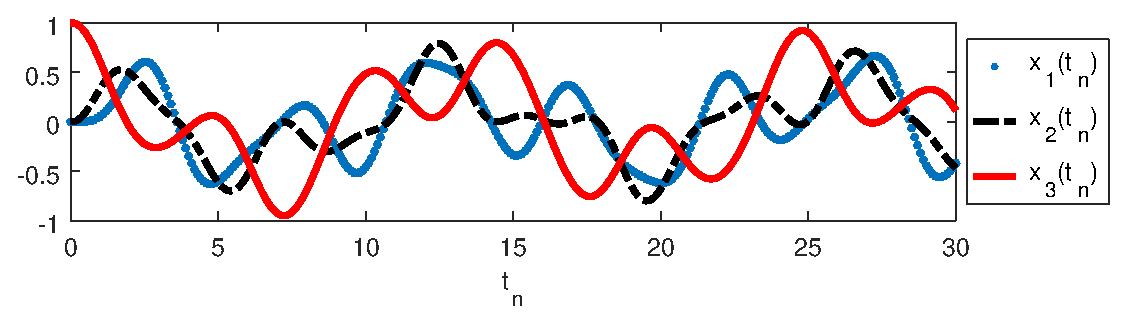
\includegraphics[width=0.89\textwidth]{chapters/differential-eq-discreto/mfiles/segundoorder/segundooder1.eps}
         \caption{Resposta $\VECTOR{x}(t)$ do Exemplo \ref{ex:ddxPx:0}.}
         \label{fig:ex:iterativo:ddxPx:0}
     \end{figure}
